\section{Evaluation}
\label{sec:evaluation}

\subsection{Experimental Setup}
\label{sec:evaluation.setup}

We implemented our monitoring architecture for adjustable overheads by
modifying the ARM version of the gem5 simulator \cite{gem5} to support parallel
run-time monitoring. In order to explore the generality of the architecture for
different monitors, we implemented three different monitors: uninitialized
memory check (UMC), array bounds check (BC), and dynamic information flow
tracking (DIFT).  Uninitialized memory check seeks to detect loading from
memory locations that are not initialized first.  Array bounds check, as
mentioned in Section~\ref{sec:monitoring} is a monitoring scheme that aims to
detect buffer overflows where memory accesses go beyond the boundaries of an
array.  Dynamic information flow tracking is a security monitoring scheme,
which detects when information from untrusted sources is used to affect the
program control flow.  We tested our system using 12 benchmarks from SPEC
CPU2006 \cite{spec2006}. For each benchmark, we simulated for 200 million
instructions. An initial slack of 2 million cycles, which is less than 1\% of
the total execution time, is given for a 10\% target overhead. This initial
slack is scaled proportionally for other overhead targets.

\subsection{Filtering of Monitoring Events}

% Full monitoring overheads
\begin{figure}
  \begin{center}
    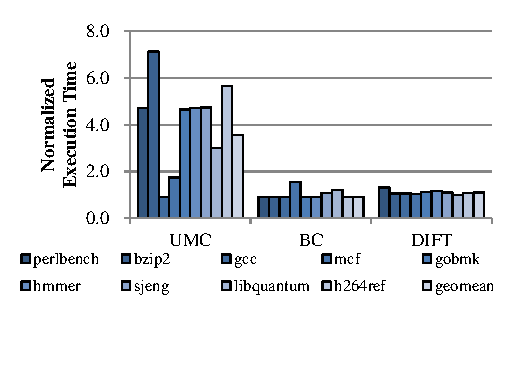
\includegraphics[width=\columnwidth]{figs/data_filtering.pdf}
    \vspace{-0.2in}
    \caption{Monitoring overheads with filtering for UMC, BC, and DIFT.}
    \label{fig:evaluation.filtering}
    \vspace{-0.1in}
  \end{center}
\end{figure}

Figure~\ref{fig:optimizations.full_mon} showed the execution time of benchmarks
with monitoring normalized to without monitoring. In this case, filtering was
not performed. UMC showed an 8x increase in execution
time on average while BC and DIFT showed average execution time increases of
21x and 14x respectively. Figure~\ref{fig:evaluation.filtering} shows the
normalized execution times with filtering enabled. We see significant
reductions in overhead for all three monitoring schemes. UMC sees normalized
execution times of 4x on average with filtering. For BC, normalized execution
times drop from 21x down to 3x. This is not surprising since in the baseline
implementation all loads and stores needed to be monitored. However, with
filtering, only loads and stores corresponding to arrays need to be forwarded.
Finally, DIFT sees the largest reduction in overheads with only 13\% overheads
on average. This is due to the fact that for our implementation of DIFT on SPEC
benchmarks, we mark data read from files as tainted. For most of these
benchmarks, this propagates to relatively few instructions. Instead, if we
targeted network or streaming applications we would expect to see a less
filtering

\subsection{Coverage with Adjustable Overheads}
Coverage and overhead budget accuracy for source, last-minute, and min-point dropping.

%\subsection{Randomness for Multi-Run Coverage}

\subsection{Area and Power Overheads}


% Area and Power Overheads
\begin{table}[tb]
  \begin{center}
    \vspace{-0.0in}
    \begin{footnotesize}
    
% Full monitoring at zero slack

\begin{tabular}{|c|c|c|}
\hline

{\bf Monitor} & {\bf Peak Power [mW]} & {\bf Runtime Power [mW]} \\ \hline\hline

UMC  & 4.7 (4.9\%) &  3.1 (8.2\%) \\ \hline
BC   & 6.9 (7.1\%) &  4.1 (10.7\%) \\ \hline
DIFT & 7.2 (7.4\%) &  4.3 (11.1\%) \\ \hline

\end{tabular}

    \end{footnotesize}
    \caption{Average power overhead for dropping hardware at a 10\% overhead
    budget. Percentages in parentheses are normalized to the main core
    power.}
    \vspace{-0.2in}
    \label{tab:evaluation.area_power}
  \end{center}
\end{table}

Adding the dropping hardware in order to enable adjustable overheads adds
overheads in terms of area and power. We use McPat \cite{mcpat-micro09} to get
a first-order estimate of these area and power overheads in a 40 nm technology
node. McPat estimates the main core area as 1.96 mm$^2$ and the peak power usage as
121 mW averaged across all benchmarks. The average runtime power usage was 38.2 
mW. These area and power numbers consist of the core and
L1 cache, but do not include L2 cache, memory controller, and other
peripherals. The power numbers include dynamic as well as static (leakage)
power. For the dropping hardware, the ALUs, MIRF, MIC, and
configuration tables are modeled using the corresponding objects in McPat. We
note that this is only a rough area and power result since components such as the
wires connecting these modules have not been modeled. However, this gives a
sense of the order-of-magnitude overheads involved with implementing our
approach.

For a 1 kB MIC, an additional 0.183 mm$^2$ of silicon area is needed, an
increase of 9\% of the main core area. Table~\ref{tab:evaluation.area_power}
shows the peak and runtime power overheads. The peak power is 13-19 mW, which is
11-16\% of the main core's peak power usage. The average runtime power is 8-11
mW, corresponding to 21-29\% of the main core's runtime power.

